% !TeX root = ..\..\main.tex

%TikZ picture to handle bendy arrows
%STRAIGHT ARROWS have the follwing syntax:
%\draw[-> OR <-] (0, Y-COORD) -- (4, Y-COORD) node[midway,above] {TEXT}; %sometimes 4 is replaced by 2 if arrow goes only halfway
%BENDY ARROWS have the following syntax:
%\draw[] (0, Y-COORD1) edge[out=0, in=180, <- OR ->] node[pos=0.75, above] {TEXT} (4, Y-COORD2);

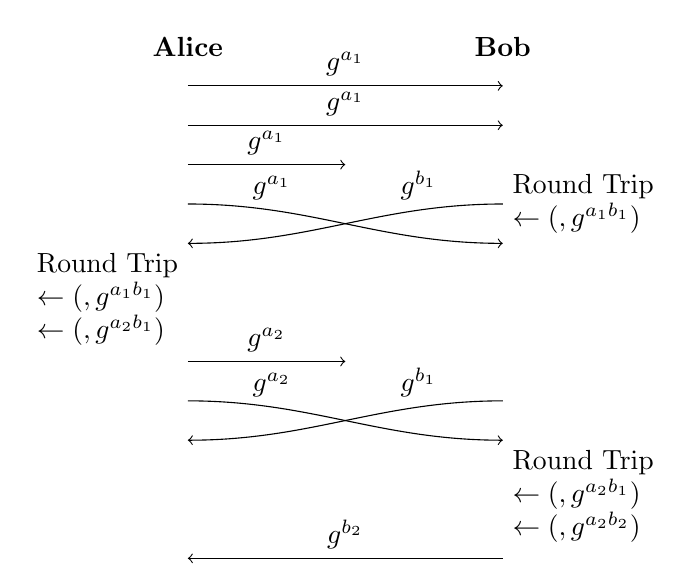
\begin{tikzpicture}
    %picture is (mostly) drawn from top to bottom depending on position of object on the left side (Alices side)
    \node (A) at (0,0) {\textbf{Alice}};
    \node (B) at (4,0) {\textbf{Bob}};
    \draw[->] (0,-.5) -- (4,-.5) node[midway,above] {$g^{a_1}$};
    \draw[->] (0,-1) -- (4,-1) node[midway,above] {$g^{a_1}$};
    \draw[->] (0,-1.5) -- (2,-1.5) node[midway,above] {$g^{a_1}$};
    %For next node: align=left to tell TikZ to align text in node left if there is a line break
    %anchor=west to place the nodes left (west) anchor at (4,-2) --> node should not be centered on (4,-2)
    \node[align=left, anchor=west] (B_RT1) at (4, -2) {Round Trip\\$\rk\gets\KDF(\rk, g^{a_1b_1})$}; 
    \draw[] (0,-2) edge[out=0, in=180, ->] node[pos=0.25, above] {$g^{a_1}$} (4,-2.5); %bend arrow with [out=0, in=180]
    %This note is anchored at north east, so the arrow points to the upper right corner 
    %(Since the node is quite high it is otherwise not clear which arrow is meant to point to it)
    \node[align=left, anchor=north east] (A_RT1) at (0, -2.5) {Round Trip\\$\rk\gets\KDF(\rk, g^{a_1b_1})$\\$\rk\gets\KDF(\rk, g^{a_2b_1})$};
    \draw[] (0, -2.5) edge[out=0, in=180, <-] node[pos=0.75, above] {$g^{b_1}$} (B_RT1);
    \draw[->] (0,-4) -- (2, -4) node[midway,above] {$g^{a_2}$};
    \node[align=left, anchor=north west] (B_RT2) at (4, -5) {Round Trip\\$\rk\gets\KDF(\rk, g^{a_2b_1})$\\$\rk\gets\KDF(\rk, g^{a_2b_2})$};
    \draw[] (0, -4.5) edge[out=0, in=180, ->] node[pos=0.25, above] {$g^{a_2}$} (4, -5);
    \draw[] (0, -5) edge[out=0, in=180, <-] node[pos=0.75, above] {$g^{b_1}$} (4, -4.5);
    \draw[<-] (0, -6.5) -- (4, -6.5) node[midway,above] {$g^{b_2}$};
\end{tikzpicture}